\chapter{Exceptions and Interrupts in Pipelined Processors}
\label{ch:exceptions_interrupts}

Le eccezioni e le interruzioni sono eventi che modificano il normale ordine di esecuzione di un programma. Nelle architetture con pipeline, la gestione di questi eventi eccezionali (eccezioni, interruzioni o fault) risulta particolarmente complessa poiché ci sono più istruzioni in esecuzione contemporaneamente in diversi stadi della pipeline.

\section{Distinzione tra Eccezione e Interruzione}
I termini "eccezione" e "interruzione" vengono spesso confusi o usati in modo intercambiabile (ad esempio, nell'ecosistema ARM si parla quasi esclusivamente di eccezioni per entrambi i casi). Tuttavia, a livello teorico, esiste una distinzione precisa basata sull'origine dell'evento:

\begin{itemize}
    \item \textbf{Eccezione (Exception):} Si riferisce generalmente a un evento interno alla CPU, generato dall'esecuzione stessa di un'istruzione. Esempi classici sono:
    \begin{itemize}
        \item Overflow in operazioni aritmetiche (es. Floating Point overflow o divisione per zero).
        \item Fault della MMU (es. Page fault, accesso non allineato in memoria).
        \item Trap o Software Interrupt (SWI), ovvero istruzioni non definite.
    \end{itemize}
    \item \textbf{Interruzione (Interrupt):} Si riferisce solitamente a un evento esterno di I/O, asincrono rispetto al flusso del programma. Esempi tipici sono:
    \begin{itemize}
        \item Richiesta da un dispositivo di I/O (es. tocco sullo schermo, ricezione di dati sulla porta seriale).
        \item Segnale di Reset o calo di alimentazione della batteria.
    \end{itemize}
\end{itemize}

\begin{remark}[Sistemi Bare-metal vs. Sistemi Operativi]
In un sistema operativo completo, le eccezioni sono spesso gestite dal kernel. Lavorando invece "bare-metal" (senza sistema operativo), come si fa abitualmente con microcontrollori RISC-V o ARM nei corsi base, il programmatore deve scrivere esplicitamente le \textit{Interrupt Service Routine} (ISR) per decidere come il processore deve reagire a ogni singolo evento (es. assegnare un valore massimo in caso di divisione per zero o ripetere l'operazione).
\end{remark}

\section{Classificazione delle Eccezioni}
Gli eventi eccezionali possono essere classificati secondo cinque categorie principali:

\subsection{Sincrone vs. Asincrone}
\begin{itemize}
    \item \textbf{Sincrone:} L'evento si verifica sempre nello stesso punto del codice se il programma viene rieseguito con gli stessi dati. Sono eccezioni generate dalle istruzioni stesse.
    \item \textbf{Asincrone:} Eventi esterni (es. timer, periferiche I/O) che non dipendono dall'istruzione in esecuzione e possono avvenire in qualsiasi momento.
\end{itemize}
\begin{example}[Emulazione floating-point tramite eccezioni sincrone]
Se un processore non possiede unità hardware per i numeri reali (Floating Point Unit), un'istruzione come \texttt{fmul.s} genererà un'eccezione di "istruzione non definita". Il programmatore può sfruttare questa eccezione sincrona per far saltare il processore a una routine software che emula la moltiplicazione reale usando le unità intere, per poi restituire il risultato e riprendere l'esecuzione.
\end{example}

\subsection{User Requested vs. Coerced (Richieste vs. Forzate)}
\begin{itemize}
    \item \textbf{User Requested:} L'utente o il programmatore richiede esplicitamente l'eccezione, in modo simile a una chiamata a procedura (es. \textit{Breakpoint} per il debugging passo-passo).
    \item \textbf{Coerced (Forzate):} Sono al di fuori del controllo del programma utente (es. page fault, hardware malfunction).
\end{itemize}

\subsection{Maskable vs. Non-maskable (Mascherabili vs. Non mascherabili)}
\begin{itemize}
    \item \textbf{Mascherabili:} L'hardware può essere configurato per ignorare (mascherare) temporaneamente la richiesta, dandole una priorità inferiore.
    \item \textbf{Non-maskable:} Eventi critici che il processore deve servire immediatamente, indipendentemente da cosa sta facendo. Un classico esempio è il segnale di calo di alimentazione (power failure).
\end{itemize}

\subsection{Within vs. Between Instructions (All'interno vs. Tra le istruzioni)}
Le eccezioni possono verificarsi \textit{all'interno} dell'esecuzione di una singola istruzione (impedendone il completamento) o \textit{tra} un'istruzione e la successiva. In architetture pipeline, la distinzione sfuma perché più istruzioni si sovrappongono.

\subsection{Resume vs. Terminate (Ripresa vs. Terminazione)}
Dopo aver gestito l'eccezione, il programma può terminare l'esecuzione oppure riprendere.
\begin{remark}[Restartable Machines e Watchdog]
Oggi quasi tutti i processori sono macchine "restartable": sono in grado di gestire un'eccezione, salvare lo stato e ripartire. Tuttavia, in sistemi \textit{safety-critical} (es. centraline automobilistiche), ripartire a tutti i costi non è sempre l'opzione migliore. Spesso si utilizza un \textbf{Watchdog Timer}, che genera un'interruzione a intervalli regolari: se il sistema è in salute, il watchdog viene "resettato" dal software; se il software si blocca, il watchdog fa scattare un reset completo del sistema.
\end{remark}

\section{Meccanismo di Gestione nella Pipeline}

Quando si verifica un'eccezione, per poter fermare e poi riavviare (Restart) l'esecuzione, la pipeline deve eseguire i seguenti passi:
\begin{enumerate}
    \item Forzare un'istruzione di \textit{trap} nella pipeline al successivo stadio di Fetch (IF).
    \item Finché la trap non viene presa, \textbf{spegnere tutte le scritture} (registri o memoria) per l'istruzione che ha causato l'eccezione e per tutte le istruzioni successive presenti nella pipeline (per evitare che i dati o gli indici si corrompano, come nel caso di autoincremento).
    \item Il controllo passa alla procedura di gestione (\textit{exception-handling procedure}), che salva immediatamente il Program Counter (PC) dell'istruzione a cui bisognerà fare ritorno.
\end{enumerate}

\subsection{Protocolli di Interruzione a confronto}
Diversi processori gestiscono il salto all'Interrupt Service Routine (ISR) in modo diverso.

\subsubsection{Architettura 80x86 (Hardware Vectoring)}
\begin{enumerate}
    \item Il dispositivo esterno invia la richiesta. La CPU rileva l'interruzione.
    \item La CPU legge il numero di identificazione $N$ (Interrupt Type) dal bus.
    \item Salva \textbf{automaticamente} nello stack il Processor Status Word (PSW), il Code Segment (CS) e l'Instruction Pointer (IP). Tutti gli altri registri usati dall'utente devono essere salvati manualmente.
    \item Azzera i flag delle interruzioni per disabilitare altre interruzioni esterne.
    \item Usa $N$ come indice per cercare nella \textbf{Interrupt Vector Table (IVT)} l'indirizzo a cui saltare.
\end{enumerate}

\subsubsection{Architettura ARM}
Simile all'80x86, usa una Interrupt Vector Table ed $N$, ma è più "gentile" con il programmatore: salva automaticamente nello stack un \textit{frame} di \textbf{8 registri} (secondo le standard ABI), tra cui il Program Counter e il Processor Status Register. Aggiorna i flag e salta all'indirizzo dell'ISR ricavato dalla tabella.

\subsubsection{Architettura RISC-V}
Il RISC-V, nella sua implementazione base, non possiede una Interrupt Vector Table hardware automatica con indice $N$.
\begin{enumerate}
    \item Salva il PC corrente e la \textbf{causa dell'eccezione} in due registri speciali dedicati.
    \item Salta a un singolo indirizzo predefinito (\textit{exception handler address}).
    \item È compito dell'utente/programmatore scrivere un blocco di codice (\texttt{switch/case}) in questo handler che legga il registro della causa e chiami la corretta funzione software (es. divisione per zero, timer, ecc.).
\end{enumerate}

\section{Eccezioni Precise e Imprecise}
Un processore possiede \textbf{eccezioni precise} se, all'arresto della pipeline per un'eccezione, si garantisce che:
\begin{itemize}
    \item Tutte le istruzioni precedenti a quella che ha scatenato l'eccezione sono state completate.
    \item Nessuna delle istruzioni successive è stata completata o ha modificato in modo permanente lo stato della macchina (possono essere riavviate da zero).
\end{itemize}
Garantire eccezioni precise è complesso quando si usano istruzioni multi-ciclo, specialmente con esecuzione fuori ordine (\textit{out-of-order completion}).

\begin{example}[Completamento fuori ordine e Stato Impreciso]
Consideriamo il seguente frammento di codice con istruzioni Floating Point, che tipicamente impiegano molti più cicli delle istruzioni intere (es. 24 cicli per la divisione):
\begin{verbatim}
fdiv.d f0, f2, f4   // Richiede molti cicli
fadd.d f10, f10, f8 // Termina prima della fdiv
fsub.d f12, f12, f14 
\end{verbatim}
Non essendoci dipendenze sui dati, \texttt{fadd.d} e \texttt{fsub.d} termineranno \textbf{prima} di \texttt{fdiv.d}. Se durante \texttt{fsub.d} si verifica un'eccezione, ci troviamo in uno stato impreciso: la \texttt{fdiv.d} (precedente) non è completa, ma la \texttt{fadd.d} (successiva) ha già sovrascritto il registro \texttt{f10}.
\end{example}

\textbf{Soluzioni possibili per le eccezioni imprecise:}
\begin{itemize}
    \item Accettare le eccezioni imprecise (sconsigliato).
    \item Fornire una modalità "lenta ma precisa" e una "veloce ma imprecisa" (eseguendo una sola operazione FP alla volta).
    \item Analizzare in anticipo (early determine) se le unità FP provocheranno eccezioni, frenando il fetch.
    \item \textbf{Bufferizzazione (Commit Stage):} Inserire i risultati temporanei in un buffer e scriverli permanentemente nei registri (fase di Write-Back) solo quando tutte le istruzioni precedenti sono state completate con successo. Questa è la strategia principale nei processori moderni (superscalari).
\end{itemize}

\section{Complicazioni nella Pipeline e Ordine delle Eccezioni}

Nel RISC-V base, i vari stadi della pipeline possono generare eccezioni differenti:
\begin{table}[H]
    \centering
    \begin{tabular}{|l|l|}
        \hline
        \textbf{Stadio della Pipeline} & \textbf{Causa dell'eccezione} \\ \hline
        \textbf{IF} (Instruction Fetch) & Page fault sull'istruzione, accesso non allineato, violazione protezione. \\ \hline
        \textbf{ID} (Instruction Decode) & Opcode indefinito o illegale. \\ \hline
        \textbf{EX} (Execution) & Eccezione aritmetica (es. overflow). \\ \hline
        \textbf{MEM} (Memory) & Page fault sui dati, accesso non allineato, violazione protezione. \\ \hline
        \textbf{WB} (Write Back) & Nessuna (lo stadio non genera eccezioni). \\ \hline
    \end{tabular}
    \caption{Sorgenti di eccezione nei vari stadi della pipeline RISC-V.}
\end{table}

A causa dell'avanzamento parallelo, possono presentarsi due problematiche critiche:

\subsection{Eccezioni Contemporanee}
Un'istruzione precedente si trova nello stadio MEM e va in fault, e un'istruzione successiva si trova nello stadio EX e va in fault contemporaneamente nello stesso ciclo di clock.
% FIGURA DA INSERIRE QUI
% Fonte: Slide 22 (Contemporary exceptions)
% Descrizione: Diagramma con fld nello stadio MEM e fadd.d nello stadio EX, con cerchi rossi che indicano le eccezioni contemporanee.
\begin{figure}[H]
    \centering
    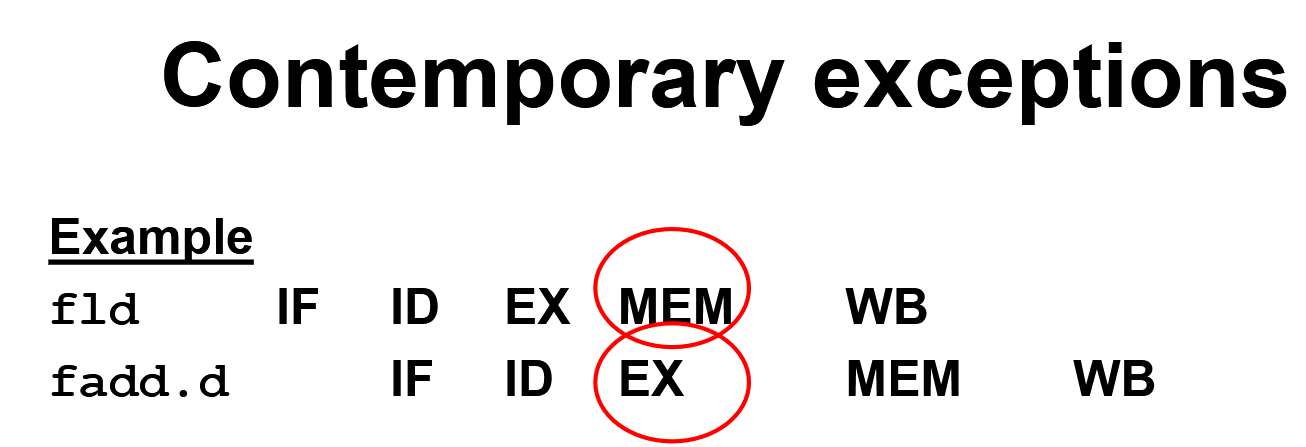
\includegraphics[width=0.8\textwidth]{capitoli/07_pipelining_exceptions/images/contemporary_exceptions}
    \caption{Eccezioni contemporanee in stadi diversi della pipeline.}
    \label{fig:contemporary_exceptions}
\end{figure}
La strategia prevede di processare sempre l'eccezione dell'istruzione "più vecchia" (quella entrata per prima, in questo caso la \texttt{fld}).

\subsection{Eccezioni in ordine inverso}
Un'istruzione successiva genera un'eccezione in uno stadio "precoce" (es. IF) prima che un'istruzione precedente generi un'eccezione in uno stadio "tardivo" (es. MEM).
% FIGURA DA INSERIRE QUI
% Fonte: Slide 23 (Exception order)
% Descrizione: Diagramma con fld (stadio MEM) che fa fault dopo che la fadd.d (stadio IF) ha già fatto un instruction page fault nel ciclo precedente.
\begin{figure}[H]
    \centering
    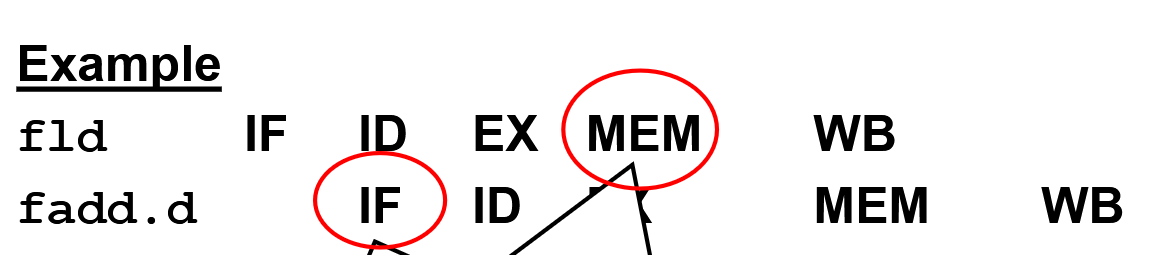
\includegraphics[width=0.8\textwidth]{capitoli/07_pipelining_exceptions/images/exception_order.png}
    \caption{Eccezioni che si verificano in ordine opposto rispetto alle istruzioni.}
    \label{fig:exception_order}
\end{figure}

\textbf{Soluzione per le pipeline RISC:}
\begin{itemize}
    \item Ad ogni istruzione viene associato uno \textbf{status flag} (o vettore di flag) che viaggia con essa nella pipeline.
    \item Se un'istruzione causa un'eccezione, non viene interrotto subito il processore, ma viene settato il suo status flag.
    \item Un'istruzione con il flag settato procede, ma le viene inibito l'accesso in scrittura (niente side-effect sulla memoria o sui registri).
    \item Solo quando l'istruzione raggiunge l'ultimo stadio (commit/WB), il processore controlla il flag. Se è settato, solleva ufficialmente l'eccezione, garantendo l'ordine cronologico del programma originale.
\end{itemize}

\subsection{Altre Complicazioni del Set di Istruzioni}
\begin{itemize}
    \item \textbf{Modifiche di stato pre-commit:} Istruzioni come quelle con indirizzamento ad \textit{autoincremento} modificano lo stato (i registri indice) prima del completamento dell'istruzione. Se abortite, lasciano uno stato alterato, costringendo il processore a logiche di \textit{roll-back} molto complesse per ripristinare il valore precedente dell'indice.
    \item \textbf{Condition Codes (Flag di stato):} Presenti in ARM e 80x86 (ma assenti in RISC-V). Causano data hazards impliciti, costringono al salvataggio e ripristino durante un'eccezione e complicano il riempimento dei \textit{branch delay slot}.
    \item \textbf{Istruzioni complesse (CISC):} Sono difficili da pipelinare mantenendo stadi di lunghezza costante. Spesso si risolve pipelinando le \textit{microistruzioni} che compongono l'istruzione complessa.
\end{itemize}